\section{Results}

Figures \ref{fig:sim_corner} shows that the drones suyccsessfully manages to safely fly around a corner and into a tight corridor. An object is present in the blind-spot around the corner. The drone manages to take a sligth detour to accure new information about the corridor before it flys into it. This ensures that it avoids the obstacle. In the corridor the drone reduces its speed as the wide range of the radar sensors makes it hard to distinguish walls from the safe area in-between. Reducing the speed gives the drone more time to acquire new data and make a new plan. 

Figures \ref{fig:squeeze} shows that the drone manages to avoid obstacles in its path, but if it has a choice then it might avoid the obstacle on a sub-optimal side. In this case, the drone luckily managed to squeeze through the opening by flying a bit back and gathering new sensor-data showing that it is safe to fly through the opening. If the opening was a bit smaller then the drone would have been stuck on the wrong side of the obstacle. In figure \ref{fig:squeeze31} it is quite obvious that the drone should rather go to the right side as this side seems a lot safer with the current information. This would require increasing the time horizon past the distance that we care about in the constraint. Choosing a path that has low risk in the future could avoid these situations. How to tune low risk path against mission progress is not clear and requires further investigation.

This control strategy is unable to avoid large convex areas such as the one in figure \ref{fig:convex_obstacle}. Figure \ref{fig:convex_corner} shows another example of an convex area where the drone gets stuck. This does at first sight not look convex, as there is only one square obstacle in the way. But it turns out that it is a convex area as the path bends from going straight down to going left around where the obstacle is present. In figure \ref{fig:convex_corner2} the drone has passed on the outside of the obstacle, but as it has to fly around another corner before it can make significant process it decides to fly back towards the path. 

\begin{figure*}
\begin{subfigure}[t]{0.3\textwidth}

\includegraphics[width=\textwidth]{Figures/Simulation/initial.eps}
\caption{t=0. The initial plan of the drone with the only the initial sensor signals}
\label{fig:sim_t0}
\end{subfigure}
\,
\begin{subfigure}[t]{0.3\textwidth}
\includegraphics[width=\textwidth]{Figures/Simulation/t19.eps}
\caption{t=19.The drone converges gradually towards the planned path.}
\label{fig:sim_t19}
\end{subfigure}
\,
\begin{subfigure}[t]{0.3\textwidth}

\includegraphics[width=\textwidth]{Figures/Simulation/t31_before_turn.eps}
\caption{t=31. The drone is tasked to fly around the corer. To drone plans to make a large turn to avoid flying straight into unknown territory. }
\label{fig:sim_t31}
\end{subfigure}\\
\begin{subfigure}[t]{0.3\textwidth}

\includegraphics[width=\textwidth]{Figures/Simulation/t45.eps}
\caption{t=45. The spread of the radar sensors makes it difficult to distinguish walls and obstacles from the narrow corridor. }
\label{fig:sim_t45}
\end{subfigure}
\,
\begin{subfigure}[t]{0.3\textwidth}

\includegraphics[width=\textwidth]{Figures/Simulation/t51_half_speed.eps}
\caption{t=51. The speed is reduced to the half to slowly approach the potentially dangerous area.}
\label{fig:sim_t51}
\end{subfigure}
\begin{subfigure}[t]{0.3\textwidth}

\includegraphics[width=\textwidth]{Figures/Simulation/t68_is_opening.eps}
\caption{t=68. New radar data is acquired showing a potential opening. }
\label{fig:sim_t68}
\end{subfigure}\\
\begin{subfigure}[t]{0.3\textwidth}

\includegraphics[width=\textwidth]{Figures/Simulation/t81_nominal.eps}
\caption{t=81. The drone continuous with nominal speed towards the opening.}
\label{fig:sim_t81}
\end{subfigure}
\,
\begin{subfigure}[t]{0.3\textwidth}

\includegraphics[width=\textwidth]{Figures/Simulation/t95_home_free.eps}
\caption{t=95.}
\label{fig:sim_t95}
\end{subfigure}
\,
\begin{subfigure}[t]{0.3\textwidth}

\includegraphics[width=\textwidth]{Figures/Simulation/final_route_superimposed.eps}
\caption{The final route of the drone with the actual obstacles superimposed on the radar map. There was a hidden obstacle right around the corner that the drone managed to avoid.}
\label{fig:sim_final}
\end{subfigure}
\caption{The black block marks the position of the drone. The black line shows the planned path. The drone is tasked to fly around the corner.}
\label{fig:sim_corner}
\end{figure*}


\begin{figure*}
\begin{subfigure}[t]{0.24\textwidth}
\includegraphics[width=\textwidth]{Figures/squeeze/t31_blocking_obstacle.eps}
\caption{t=31. An obstacle is blocking the path, the drone decides to avoid to the left.}
\label{fig:squeeze31}
\end{subfigure}
\,
\begin{subfigure}[t]{0.24\textwidth}

\includegraphics[width=\textwidth]{Figures/squeeze/t61_quarter_Speed_wring_dir.eps}
\caption{t=61.The opening is too tight so the flys away form the path with minimal speed.}
\label{fig:squeeze61}
\end{subfigure}
\,
\begin{subfigure}[t]{0.24\textwidth}

\includegraphics[width=\textwidth]{Figures/squeeze/t98_squeeze_through.eps}
\caption{t=91. An opening is found and the drone manages to squeeze through. }
\label{fig:squeeze98}
\end{subfigure}
\,
\begin{subfigure}[t]{0.24\textwidth}

\includegraphics[width=\textwidth]{Figures/squeeze/final_path.eps}
\caption{The final path the drone followed. }
\label{fig:squeeze_final}
\end{subfigure}
\caption{The drone is tasked to fly straight down. It manages to avoid the obstacle.}
\label{fig:squeeze}
\end{figure*}

\begin{figure*}
\begin{subfigure}[t]{0.3\textwidth}
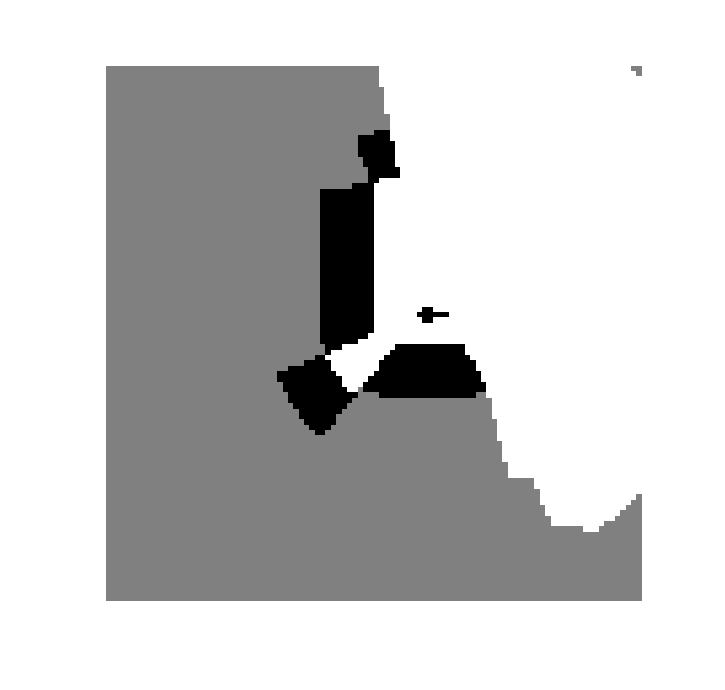
\includegraphics[width=\textwidth]{Figures/convex_corner/t71_trying_fly_around.eps}
\caption{t=71. An obstacle is blocking the path, the drone tries to fly around it to the right.}
\label{fig:convex_corner1}
\end{subfigure}
\,
\begin{subfigure}[t]{0.3\textwidth}
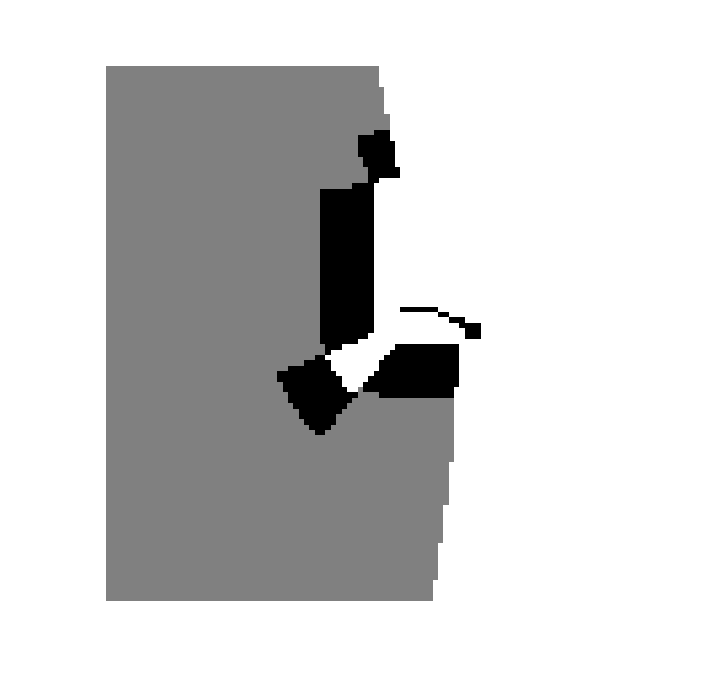
\includegraphics[width=\textwidth]{Figures/convex_corner/t111_gives_up.eps}
\caption{t=111. The drone gives up as flying back to the path is preferable.}
\label{fig:convex_corner2}
\end{subfigure}
\,
\begin{subfigure}[t]{0.3\textwidth}
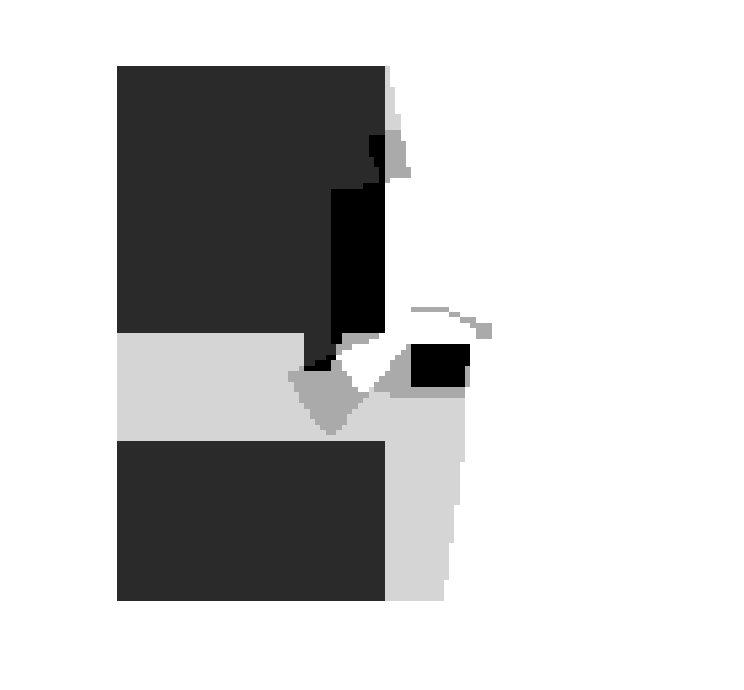
\includegraphics[width=\textwidth]{Figures/convex_corner/superimposed_obstacles_map.eps}
\caption{A superimposed map showing that there was a path around the obstacle that the drone did not find. }
\label{fig:convex_corner3}
\end{subfigure}
\caption{The drone is tasked to fly around the corner. Obstacles blocking the corner can create convex hulls where the drone gets stuck.}
\label{fig:convex_corner}
\end{figure*}

\begin{figure}
    \centering
    
\includegraphics[width = \linewidth]{Figures/convex_obstacle.eps}
    \caption{The drone gets stuck in convex obstacles. The true obstacle positions are superimposed on the map.}
    \label{fig:convex_obstacle}
\end{figure}



